% !Mode:: "TeX:UTF-8"

Neste capítulo serão apresentados os testes para as funcionalidades disponíveis ao administrador após a instalação do sistema, referentes ao registro de operadores e gerenciamento das funções disponíveis no sistema.

\section{Operadores}\label{sec:operadores}

Ao logar-se como administrador, é possível ver o menu de funções. Ao clicar em \textit{Operadores}, duas possibilidades serão mostradas: \textit{Listar} e \textit{Registrar}.


\subsection{Registrar operadores}\label{subsec:cadEntidades}

Ao acessar o menu, será carregada uma página, como mostra a figura \ref{fig:registroop}.

\begin{figure}[ht]
     \centering
     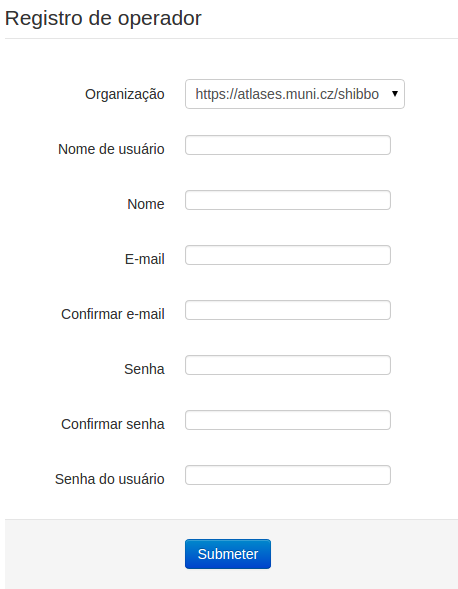
\includegraphics[scale=0.6]{images/registroop.png}
     \caption{Registro de Operador}
     \label{fig:registroop}
\end{figure}

\subsubsection{Entradas}

\begin{itemize}

	\item Submeter com os campos vazios 
	\item Preencher e-mail sem formatação (ex. operador.com)
	\item Preencher todos os campos, menos confirmação de e-mail e confirmação de senha
	\item Preencher confirmação de e-mail e confirmação de senha com entradas diferentes dos campos de e-mail e senha
	\item Submeter formulário com a senha do administrador errada
	\item Submeter um segundo formulário com o nome de usuário igual ao nome do primeiro operador cadastrado
	\item Submeter o formulário corretamente, com confirmações de e-mail e senha idênticos aos originais, senha de usuário correta, formatação do e-mail válida (operador@teste.com) e nenhum campo em branco
	
\end{itemize}

\subsubsection{Saídas}

\begin{itemize}

	\item Devem aparecer alertas ao lado de cada campo preenchido de forma (formatação) inválida ou submetido em branco
	\item Deve aparecer um alerta de erro se o e-mail e senha de confirmação não forem idênticos aos originais
	\item Deve aparecer um alerta de "senha incorreta" se a senha do usuário estiver errada
	\item Deve aparecer um alerta de "operador já cadastrado" ao tentar cadastrar operadores com nomes de usuário idênticos
	\item Se os dados estiverem todos preenchidos de forma correta, sem repetição com outro membro já cadastrado e com senha de usuário correta, deve aparecer uma mensagem de "Sucesso" e o usuário deve ser redirecionado para a tela de listagem de operadores
	
\end{itemize}

\subsubsection{Dependência de casos de teste}
Não há dependência com nenhum outro caso de teste.

\subsection{Listar Operadores}

No menu \textit{Operadores $>$ Listar}, o usuário deve ser capaz de visualizar os operadores já cadastrados.
Na página aparecerá uma lista com todos os operadores, semelhante à imagem \ref{fig:listarop}.
Na aba onde são listados deve ser possível ver \textit{Nome de usuário, Nome, Email, Organização e Ação} de cada operador registrado. As ações possíveis são:

\begin{itemize}

	\item \textbf{Excluir operador(}\begin{wrapfigure} 
\includegraphics[height=10]{images/iconedelete2} \end{wrapfigure} \textbf{):} Remove o operador do banco. O mesmo não poderá mais logar no sistema.
	\item \textbf{Editar operador(}\begin{wrapfigure} 
\includegraphics[height=10]{images/iconeeditar} \end{wrapfigure} \textbf{):} É mostrada uma tela onde é possível alterar alguns dados do operador.
	
\end{itemize}

\subsubsection{Entradas}

\begin{itemize}

	\item Clicar na ação "Excluir operador". Submeter a solicitação passando uma senha inválida de administrador
	\item Clicar na ação "Excluir operador". Submeter a solicitação passando uma senha válida de administrador
	\item Clicar na ação "Editar operador". Alterar os dados do usuário utilizando os casos de teste 4.1.1.1
	
\end{itemize}

\subsubsection{Saídas}

\begin{itemize}

	\item Deve aparecer um alerta de erro ao tentar excluir um operador com a senha errada. Ao acessar novamente a listagem de operadores, os dados deste operador ainda devem estar lá
	\item Deve aparecer uma mensagem de sucesso ao fornecer a senha correta e o usuário deve ser redirecionado para a listagem de operadores, onde os dados do operador excluído não devem mais aparecer
	
\end{itemize}

\subsubsection{Dependência de casos de teste}
Há dependência com o caso de teste 4.1.1.1 na página 9.

\begin{figure}[ht]
     \centering
     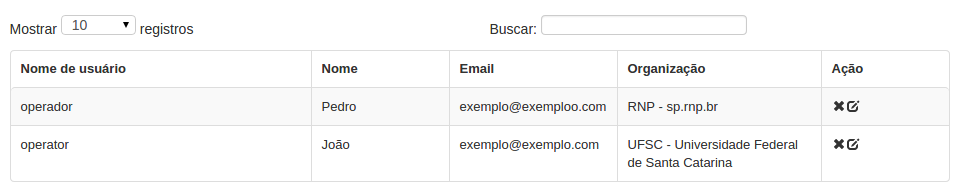
\includegraphics[scale=0.5]{images/listarop.png}
     \caption{Listagem de Operadores}
     \label{fig:listarop}
\end{figure}

\subsection{Editar Operadores}
    Deve ser possível editar todo e qualquer operador da listagem, seguindo as entradas e inspecionando as saídas especificadas no caso de teste 4.1.1.Tf

\section{SMTP}

\subsection{Registrar SMTP}

SMTP(do inglês \textit{Simple Mail Transfer Protocol}) é o protocolo padrão para envio de e-mails através da Internet. É necessário configurar o e-mail e as mensagens automáticas que devem ser enviadas para o mesmo caso ocorra algum erro ou algum certificado seja emitido.
Para registrar o SMTP deve-se ir ao ícone \textit{SMTP $>$ Registrar}. Será carregada uma página, como mostra a figura \ref{fig:smtp}. É escolha do administrador utilizar uma autenticação extra ou cadastrar sem autenticação (quando não é preciso inserir login e senha do e-mail). 

\subsubsection{Entradas}
Para testar sem autenticação:

\begin{itemize}
	\item Submeter com os campos vazios 
	\item Preencher e-mail sem formatação (ex. operador.com)
	\item Preencher Host smtp e Porta errados
	\item Submeter formulário com a senha do administrador errada
	\item Submeter formulário com nome de usuário do administrador errado
	\item Submeter ao menos dois formulários de maneira correta, com confirmação de senha idêntica à original, senha de usuário correta, formatação do e-mail válida (operador@teste.com) e nenhum campo em branco. Um formulário deve assinalar o campo "Mandar um email teste" e o outro, não
\end{itemize}

Para testar para cada tipo de autenticação (Nenhuma, Usuário e Senha, Plain e CRAMD5):

\begin{itemize}
	\item Submeter com os campos vazios 
	\item Preencher e-mail sem formatação (ex. operador.com)
	\item Preencher Host smtp e Porta errados
	\item Preencher todos os campos, menos confirmação de senha
	\item Preencher confirmação de senha com entrada diferente do campos original
	\item Submeter formulário com a senha do administrador errada
	\item Submeter formulário com nome de usuário do administrador errado
	\item Submeter ao menos dois formulários de maneira correta, com confirmação de senha idêntica à original, senha de usuário correta, formatação do e-mail válida (operador@teste.com) e nenhum campo em branco. Um formulário deve assinalar o campo "Mandar um email teste" e o outro, não
	\item Submeter para cada formulário, com e sem a opção de "Mandar um e-mail teste", um tipo diferente de protocolo criptográfico (Nenhum, SSL e TLS)
\end{itemize}

\begin{figure}[ht]
     \centering
     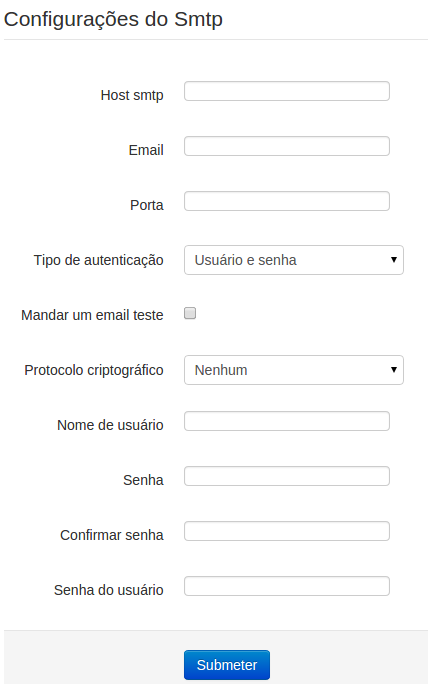
\includegraphics[scale=0.6]{images/smtp.png}
     \caption{Registrar SMTP}
     \label{fig:smtp}
\end{figure}

\subsubsection{Saídas}

\begin{itemize}
    \item Devem aparecer alertas ao lado de cada campo preenchido de forma (formatação) inválida ou submetido em branco
	\item Deve aparecer um alerta de erro se a senha de confirmação não for idêntica à original
	\item Deve aparecer um alerta de "senha incorreta" se a senha do usuário estiver errada
	\item Se os dados estiverem todos preenchidos de forma correta, para cada e-mail onde a opção "Mandar um e-mail teste" foi assinalada, o usuário deve receber um e-mail de notificação no prazo de 30 minutos
	\item Se os dados estiverem todos preenchidos de forma correta, para cada e-mail onde a opção "Mandar um e-mail teste" não foi assinalada, o usuário não deve receber um e-mail de notificação na caixa de entrada
\end{itemize}

\subsubsection{Dependência de casos de teste}
Não há dependência com nenhum outro caso de teste.

\subsection{Configurar Mensagens}

Nesta parte do sistema o administrador deve configurar as mensagens que serão enviadas para o seu e-mail de forma automática quando algum evento acontecer. Para configurar as mensagens do SMTP deve-se ir ao ícone \textit{SMTP $>$ Configurar mensagens}. O usuário deve configurar o assunto e o conteúdo do e-mail para cada um dos eventos possíveis (erros e emissões de LCR e Certificados):

\subsubsection{Entradas}
\begin{itemize}
	\item Submeter formulário com a senha do administrador errada
	\item Submeter formulário com novas mensagens, com o campo de assunto do e-mail vazio
	\item Submeter formulário com assuntos de e-mail, porém com corpo de e-mail vazio
	\item Submeter formulário com assunto e corpo do e-mail somente com números, sem palavras ou texto válidos
	\item Submeter formulário correto, com senha de usuário válida e sem campos em branco
	\item Executar as funcionalidades relacionadas às mensagens para confirmar a corretude destas via e-mail
\end{itemize}

\subsubsection{Saídas}
\begin{itemize}
    \item Deve aparecer um alerta de "senha incorreta" se a senha do usuário estiver errada
    \item Devem aparecer alertas ao lado de cada campo preenchido de forma inválida (somente números) ou submetido em branco
	\item Ao submeter o formulário correto e executar as funcionalidades correspondentes, deve-se acessar o e-mail e as mensagens e respectivos assuntos devem ser conferidos e devem estar idênticos aos originais submetidos no sistema
\end{itemize}

\subsubsection{Dependência de casos de teste}
Há dependência com o caso de teste 4.2.1.1 na página 12.

\section{Modelos}

Esta é a parte onde deve-se configurar o modelo das LCRs e dos Certificados que serão emitidos.

\subsection{LCR}

Para configurar o template de LCR, deve-se selecionar o menu \textit{Modelos $>$ LCR}. Aparecerá uma tela igual à imagem \ref{fig:modelolcr} mostrada abaixo. Este template configura o período de validade de cada LCR. Caso o administrador queira que uma LCR nova seja emitida toda vez que a última vence, ele deve aceitar a opção "Emissão automática".

\begin{figure}[ht]
     \centering
     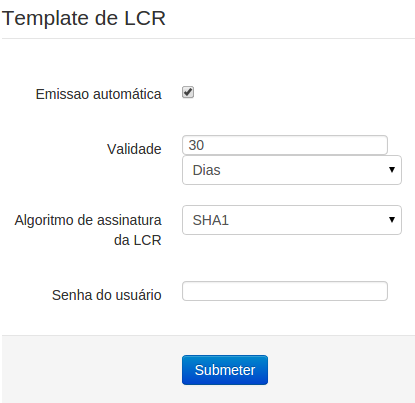
\includegraphics[scale=0.5]{images/modelolcr.png}
     \caption{Modelo de LCR}
     \label{fig:modelolcr}
\end{figure}

\subsubsection{Entradas}

\begin{itemize}

	\item Submeter com os campos vazios 
	\item Submeter formulário com a senha do administrador errada
	\item Submeter formulário com número de validade gigante (1234567890123456789)
	\item Submeter formulário com número de validade igual a zero (0)
	\item Submeter o formulário corretamente, com senha de usuário correta e nenhum campo em branco
	\item Testar cada uma das entradas acima pelo menos uma vez para cada algoritmo de assinatura diferente
\end{itemize}

\subsubsection{Saídas}

\begin{itemize}

	\item Devem aparecer alertas ao lado de cada campo preenchido de forma inválida ou submetido em branco
	\item Deve aparecer um alerta de "senha incorreta" se a senha do usuário estiver errada
	\item Se os dados estiverem todos preenchidos de forma correta deve aparecer uma mensagem de "Sucesso" e o usuário deve ser redirecionado para a tela inicial
	
\end{itemize}

\subsubsection{Dependência de casos de teste}
Não há dependência com nenhum outro caso de teste.

\subsection{Certificado}

O administrador deve clicar em \textit{Modelos $>$ Certificado}. Será mostrada uma tela como na figura \ref{fig:modelocert}. Os atributos que já vêm marcados por default não devem ser alterado, pois estes esão registrados na DPC (Declaração de Políticas do Certificado). Se algum atributo novo for configurado, ou algum deixar de existir, o OID (Object Identifier) da DPC deve ser alterado na seção "Políticas de Certificado". Quanto à validade, esta não é a validade do certificado que será emitido, e sim a validade das configurações do mesmo.


\begin{figure}[ht]
     \centering
     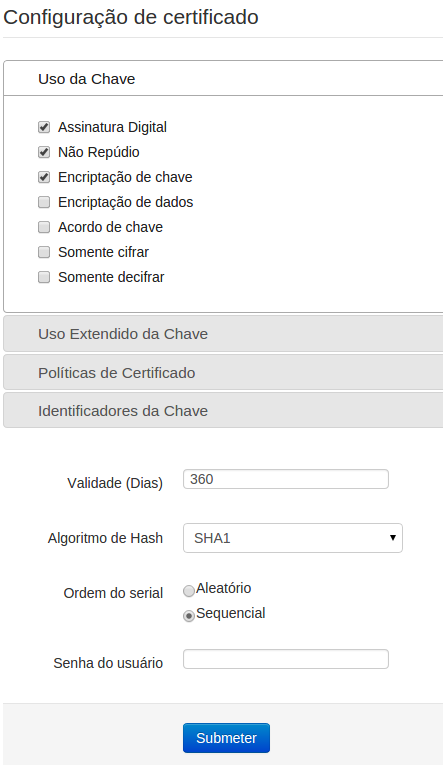
\includegraphics[scale=0.5]{images/modelocert.png}
     \caption{Modelo de Certificado}
     \label{fig:modelocert}
\end{figure}

\subsubsection{Entradas}
\begin{itemize}
	\item Submeter com os campos vazios 
	\item Submeter formulário com a senha do administrador errada
	\item Submeter formulário com número de validade gigante (1234567890123456789)
	\item Submeter o formulário corretamente, com senha de usuário correta, nenhum campo em branco e nenhum campo avançado preenchido
	\item Submeter o formulário corretamente, preenchendo todos os campos avançados disponíveis (Uso extendido da Chave, Políticas de Certificado e Identificadores da Chave)
	\item Submeter formulários com vários tipos de combinação para o Uso da Chave
	\item Submeter ao menos um formulário correto para ordem Aleatória e um para ordem Sequencial
	\item Testar cada uma das entradas acima pelo menos uma vez para cada algoritmo de assinatura diferente
\end{itemize}


\subsubsection{Saídas}

\begin{itemize}

	\item Devem aparecer alertas ao lado de cada campo preenchido de forma (formatação) inválida ou submetido em branco (para os campos com valor obrigatório)
	\item Deve aparecer um alerta de "senha incorreta" se a senha do usuário estiver errada
	\item Nenhum erro deve ser reportado se o usuário deixar os campos avançados em branco
	\item Nenhum erro deve ser reportado para as seleções de Uso da Chave, uma vez que o sistema deve suportar qualquer combinação
	\item Se os dados estiverem todos preenchidos de forma correta deve aparecer uma mensagem de "Sucesso" e o usuário deve ser redirecionado para a tela inicial
	
\end{itemize}

\subsubsection{Dependência de casos de teste}
Não há dependência com nenhum outro caso de teste.

\section{LCR}

Esta é a parte do sistema que permite que o administrador emita uma Lista de Certificados Revogados até o momento e faça o Download da LCR que desejar.

\subsection{Emitir}

Para emitir uma LCR é preciso acessar o menu \textit{LCR $>$ Emitir}. Basta informar a senha de administrador e clicar \emph{Submeter}. O sistema vai emitir uma lista com todos os certificados revogados até o momento. Por este motivo não se faz necessário um  caso de teste específico para esta funcionalidade, basta tentar executar a ação duas vezes, passando uma senha de usuário válida e uma inválida. Ao receber uma senha válida, o sistema deve mostrar uma mensagem de "Sucesso" e emitir a LCR, que será automaticamente baixada pelo navegador. Ao receber uma senha inválida, o sistema deve reportar um erro.

\subsubsection{Dependência de casos de teste}
Não há dependência com nenhum outro caso de teste.

\subsection{Download}

Para fazer o download de uma LCR é preciso acessar o menu \textit{LCR $>$ Download}. É possível fazer download de duas formas diferentes, como mostra a figura \ref{fig:lcr}. 

\begin{figure}[ht]
     \centering
     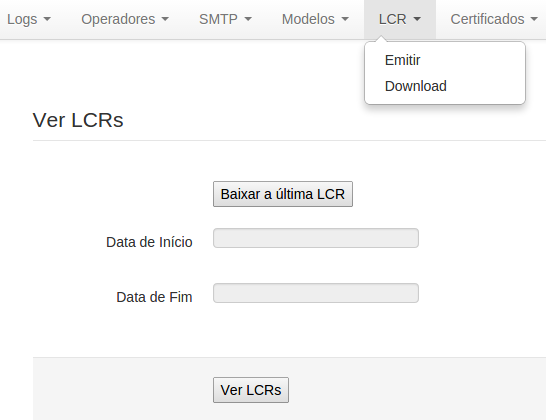
\includegraphics[scale=0.6]{images/lcr.png}
     \caption{Download de LCR}
     \label{fig:lcr}
\end{figure}

\subsubsection{Entradas}
\begin{itemize}

	\item Baixar a última LCR
	\item Preencher data de início para uma data posterior à de fim
	\item Preencher campos de data de início e fim com data do futuro
	\item Preencher só o campo de data de início, sem preencher a de fim
	\item Preencher só o campo de data de fim, sem preencher a de início
	\item Clicar em "Ver LCRs" sem preencher os campos de data de início e de fim
	\item Submeter os campos de data de início e fim corretamente ao clicar em "Ver LCRs'
	
\end{itemize}

\subsubsection{Saídas}

\begin{itemize}

	\item Devem aparecer alertas ao lado de cada campo preenchido de forma inválida (datas do futuro ou com período errado) ou submetido em branco
    \item A última LCR deve ser baixada automaticamente ao clicar no botão
    \item As LCRs por período devem ser baixadas automaticamente ao clicar no botão "Ver LCRs" com os campos preenchidos de maneira válida
	
\end{itemize}

\subsubsection{Dependência de casos de teste}
Há dependência com o caso de teste 4.4.1 na página 18.

\section{Certificados}

No menu \textit{Certificados} deve ser possível listar todos os certificados emitidos até o momento, estejam eles ativos ou revogados. Acesse o menu \textit{Certificados $>$ Listar}. Aparecerá uma tela como mostra a figura \ref{fig:listarcert}. Nesta página deve possível ver a organização e o e-mail do operador afiliado à organização responsável pela emissão do certificado, a data em que foi emitido e a data em que este irá expirar, bem como o estado em que se encontra (Ativo ou revogado). É possível realizar as seguintes ações:

\begin{itemize}

	\item \textbf{Download do certificado(}\begin{wrapfigure} 
\includegraphics[height=10]{images/iconedownload} \end{wrapfigure} \textbf{):} Ao clicar nesse ícone você faz o download do certificado selecionado.
	\item \textbf{Revogar certificado(}\begin{wrapfigure} 
\includegraphics[height=10]{images/iconedelete2} \end{wrapfigure} \textbf{):} Quando um certificado estiver ativo, este ícone irá aparecer na linha do respectivo certificado para que este possa ser revogado individualmente. Se houver necessidade de revogar mais certificados, é possível selecioná-los e revogalos de uma só vez através do ícone de revogação no canto inferior direito da imagem. 
	
\end{itemize}

\begin{figure}[ht]
     \centering
     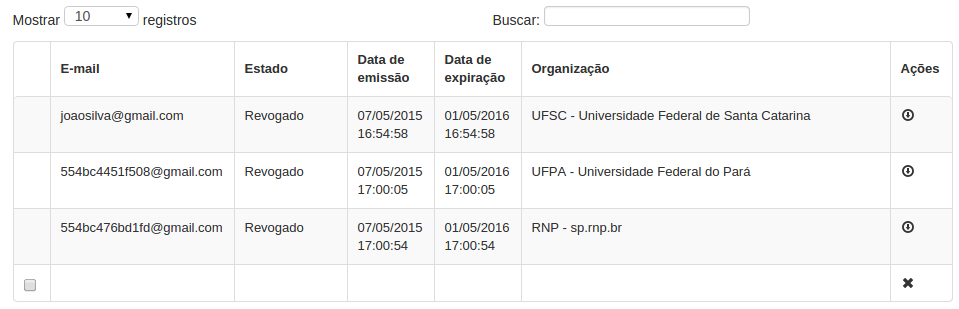
\includegraphics[scale=0.5]{images/listarcert.png}
     \caption{Listagem de certificados}
     \label{fig:listarcert}
\end{figure}

\subsubsection{Entradas}
\begin{itemize}

	\item Fazer download de cada um dos certificados 
	\item Revogar um certificado informando a senha de usuário inválida
	\item Revogar um certificado informando a senha de usuário válida
	\item Submeter o formulário para revogação em branco (sem informar o motivo da revogação)
	\item Utilizar a revogação em lotes, clicando no quadrado no canto inferior esquerdo da tabela, utilizando as mesmas entradas citadas acima
	\item Executar busca de certificado através do e-mail, fornecendo um e-mail inválido
	\item Executar busca de certificado através do e-mail, fornecendo um e-mail válido
	
\end{itemize}

\subsubsection{Saídas}

\begin{itemize}

	\item O certificado deve ser baixado imediatamente ao clicar na ação de download, podendo este ser visualizado corretamente após baixado
	\item Devem aparecer alertas ao lado de cada campo preenchido de forma inválida ou submetido em branco
	\item Ao tilizar a revogação em lotes, os certificados que já estiverem revogados não devem ser assinalados na tela
	\item A busca com e-mail inválido deve retornar um erro claro e preciso que informe ao usuário que o certificado não foi encontrado
	\item A busca com e-mail válido deve retornar os certificados emitidos para aquele e-mail
	
\end{itemize}

\subsubsection{Dependência de casos de teste}
Depende se há ou não certificados emitidos. Para este caso de teste, é necessário que o usuário emita pelo menos dois certificados seguindo os casos de teste no capítulo de Usuário Final.

\section{Backup}

Fazer um backup do sistema significa salvar toda a sua estrutura. O backup contém todas as operações realizadas até o momento. O backup do sistema de emissão de certificados ICPEdu é cifrado, pelo fato de poder haver dados sigilosos, a partir de uma senha que será escolhida pelo usuário.

\subsection{Gerar}

Para gerar o backup, basta selecionar o menu \textit{Backup $>$ Gerar}. Aparecerá uma tela igual à imagem \ref{fig:gerarbackup} mostrada abaixo. O usuário deve preencher o primeiro campo com a senha para cifrar o backup e confirmá-la no campo abaixo. É importante armazenar essa senha em local seguro, pois sem ela, será impossível restaurar o backup.

\subsubsection{Entradas}
\begin{itemize}

	\item Submeter com todos os campos em branco
	\item Submeter apenas com os dois primeiros campos em branco
	\item Submeter com senha de cifragem diferente do campo "Confirmar senha"
	\item Submeter com senha de cifragem igual à do campo "Confirmar senha", porém com senha do usuário inválida
	\item Submeter corretamente, com senha de cifragem igual à do campo "Confirmar senha" e senha do usuário válida
	
\end{itemize}

\begin{figure}[ht]
     \centering
     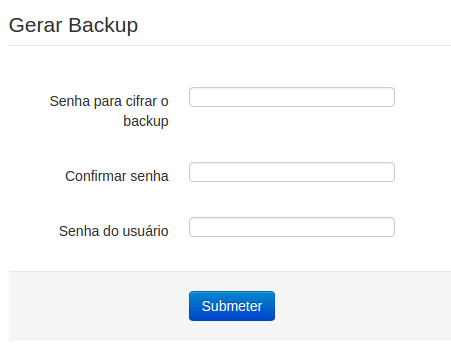
\includegraphics[scale=0.6]{images/gerarbackup.png}
     \caption{Gerar Backup}
     \label{fig:gerarbackup}
\end{figure}

\subsubsection{Saídas}

\begin{itemize}

	\item Devem aparecer alertas ao lado de cada campo preenchido de forma inválida ou submetido em branco
	\item Deve aparecer um erro que informe de forma clara e precisa ao usuário que a senha de cifragem não confere com a senha de confirmação
	\item Deve aparecer uma mensagem de senha inválida ao submeter com senha de usuário incorreta
	\item Se todos os campos estiverem corretos, o backup deve ser gerado e baixado automaticamente em extensão .bkp
	
\end{itemize}

\subsubsection{Dependência de casos de teste}
Não há dependência com nenhum outro caso de teste.

\subsection{Restaurar}

Para inserir as entradas deste caso de teste, o administrador deve entrar no sistema e clicar no menu \textit{Backup $>$ Restaurar}. Será mostrada a tela de recuperação de backup, como mostra a imagem \ref{fig:restaurarbackup}:

\begin{figure}[ht]
     \centering
     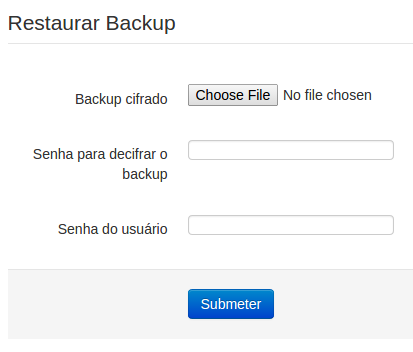
\includegraphics[scale=0.6]{images/restaurarbackup.png}
     \caption{Restaurar Backup}
     \label{fig:restaurarbackup}
\end{figure}

\subsubsection{Entradas}
\begin{itemize}

	\item Submeter um arquivo qualquer que não seja o backup do SAEC, com senha de cifragem correta
	\item Submeter o arquivo .bkp correto, com a senha de cifragem incorreta
	\item Submeter um arquivo correto, com senha de cifragem correta e senha de usuário incorreta
	\item Submeter tudo corretamente, inclusive senha de usuário
	
\end{itemize}

\subsubsection{Saídas}

\begin{itemize}

	\item Deve aparece um erro claro e preciso que informe ao usuário quando o arquivo é inválido
	\item Deve aparecer um erro que informe de forma clara e precisa ao usuário que a senha de cifragem não confere com a senha salva no banco de dados
	\item Deve aparecer uma mensagem de senha inválida ao submeter tudo corretamente, porém com senha de usuário incorreta
	\item Se todos os campos estiverem corretos, o sistema deve ser restaurado para seu estado anterior à geração do backup
	
\end{itemize}

Quanto à restauração, recomenda-se que, para melhor testar a funcionalidade, haja alguma diferença no estado do sistema entre o teste de geração e de restauração, como, por exemplo, inserir um novo operador no banco de dados através do caso de teste 4.1.1.1 da página 10. Após inserir um novo operador e restaurar o backup que foi gerado anteriormente, o sistema deve voltar ao estado onde este operador ainda não existia e, portanto, o operador não deve aparecer na listagem.

\subsubsection{Dependência de casos de teste}
Há dependência com o caso de teste 4.6.1.1 na página 21.

\section{Estatísticas}

Esta parte do sistema destina-se à mostrar as estatísticas (por tempo ou por organização) dos certificados emitidos. Deve ser possível verificar quantos certificados foram emitidos, quantos estão ativos, quantos estão revogados e quantos estão expirados.

\subsection{Total}

Acesse o menu \textit{Estatísticas $>$ Total}. Aparecerá uma tela como mostra a figura \ref{fig:estotal}. Deve ser possível ver quantos certificados já foram emitidos no total, bem como quantos ainda estão ativos e quantos já foram revogados. Logo em baixo deve ser possível clicar nas organizações e ver as estatísticas em separado de cada uma delas. Lembrando que, para poder ver a estatística de uma organização específica, é necessário possuir um operador cadastrado para ela, do contrário a organização não aparecerá na tela como mostrado na figura abaixo. Como se trata de uma funcionalidade que não requere entradas e saídas, não é necessário um plano de testes. Porém, cabe ao usuário conferir se existe estatística para toda organização que possuir operadores.

\begin{figure}[ht]
     \centering
     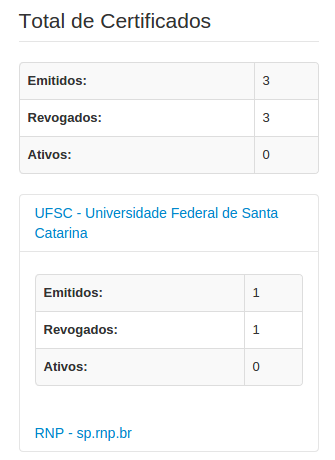
\includegraphics[scale=0.6]{images/estatisticatotal.png}
     \caption{Estatísticas total}
     \label{fig:estotal}
\end{figure}

\subsubsection{Dependência de casos de teste}
Depende se há ou não certificados emitidos. Para este caso de teste, é necessário que o usuário emita pelo menos dois certificados para duas instituições diferentes, seguinto os casos de teste no capítulo de Usuário Final.

\subsection{Procurar por tempo}

Acesse o menu \textit{Estatísticas $>$ Procurar por tempo}. Aparecerá uma tela como mostra a figura \ref{fig:estempo}.

\begin{figure}[ht]
     \centering
     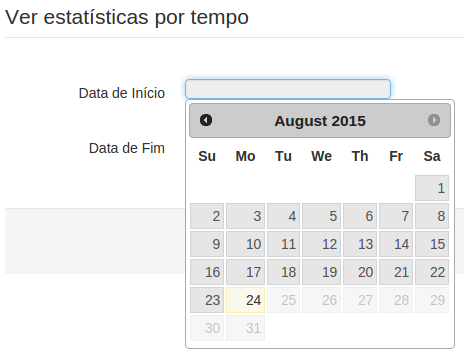
\includegraphics[scale=0.5]{images/estatisticatempo.png}
     \caption{Estatísticas por tempo}
     \label{fig:estempo}
\end{figure}

\subsubsection{Entradas}

\begin{itemize}

    \item Submeter com os campos em branco
	\item Preencher data de início para uma data posterior à de fim
	\item Preencher campos de data de início e fim com data do futuro
	\item Preencher só o campo de data de início, sem preencher a de fim
	\item Preencher só o campo de data de fim, sem preencher a de início
	\item Preencher tudo corretamente e submeter
	
\end{itemize}

\subsubsection{Saídas}

\begin{itemize}

	\item Devem aparecer alertas ao lado de cada campo preenchido de forma inválida ou submetido em branco
	\item Se os dados estiverem todos preenchidos de forma correta o usuário deve ser redirecionado para a tela de estatísticas
	
\end{itemize}

\subsubsection{Dependência de casos de teste}
Depende se há ou não certificados emitidos. Para este caso de teste, é necessário que o usuário emita pelo menos dois certificados para duas instituições diferentes, seguinto os casos de teste no capítulo de Usuário Final.

\section{Atributos}

Através do menu \textit{Atributos $>$ Mapeador de atributos} o administrador deve poder escolher quais atributos o certificado vai requerer, como mostra a figura \ref{fig:atmap}.

\begin{figure}[ht]
     \centering
     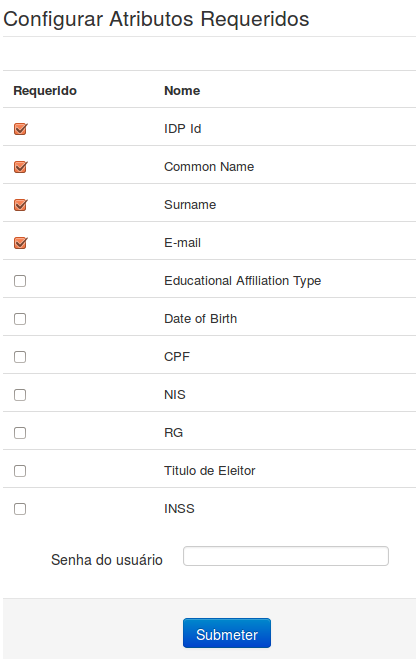
\includegraphics[scale=0.6]{images/attributesmapper.png}
     \caption{Mapeador de atributos}
     \label{fig:atmap}
\end{figure}

Para executar esta funcionalidade, é preciso somente marcar os atributos que devem aparecer obrigatoriamente no seu certificado, insirir sua senha de administrador e clicar no botão \textit{Submeter}. Por este motivo não se faz necessário um  caso de teste específico para esta funcionalidade, basta tentar executar a ação duas vezes, passando uma senha de usuário válida e uma inválida. Ao receber uma senha válida, o sistema deve mostrar uma mensagem de "Sucesso" e voltar para a página inicial.

\subsubsection{Dependência de casos de teste}
Não há dependência com nenhum outro caso de teste.

\section{Cron}

Através do menu \textit{Cron $>$ Tarefas do Cron} deve ser possível verificar as próximas tarefas agendadas para o Cron e também agendar uma nova.

\subsection{Emissão automática de LCR}

Deve ser possível verificar a próxima emissão de LCR (desde que essa tenha sido agendada automaticamente através do menu Modelos>LCR). Como não deve ser possível alterá-la, não se faz necessário um  caso de teste específico para esta funcionalidade.

\begin{figure}[ht]
     \centering
     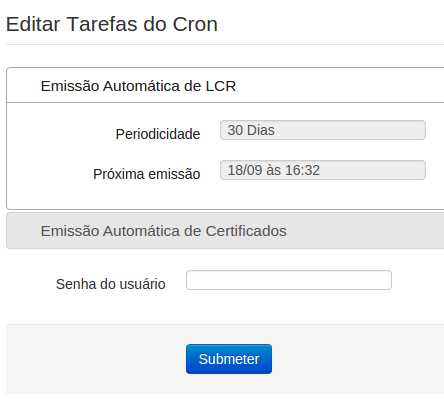
\includegraphics[scale=0.5]{images/cron.png}
     \caption{Emissão automática de LCR}
     \label{fig:cron}
\end{figure}

\subsubsection{Dependência de casos de teste}
Há dependência com o caso de teste 4.3.1.1 na página 16.

\subsection{Emissão automática de Certificados}

Deve ser possível editar as tarefas do Cron que tratam da parte de emissão de certificados pendentes. Para fazer isso, basta assinar a caixa \textit{Agendar} e inserir a periodicidade desejada, como mostra a figura \ref{fig:croncert}.

\begin{figure}[ht]
     \centering
     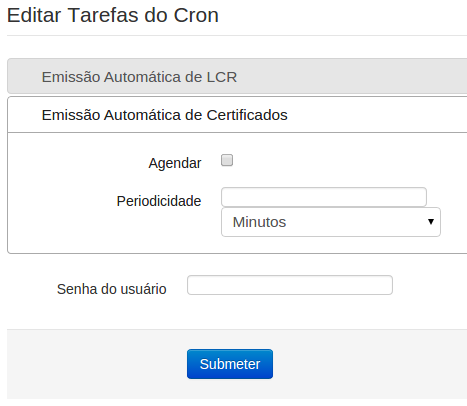
\includegraphics[scale=0.5]{images/croncert.png}
     \caption{Emissão automática de Certificados}
     \label{fig:croncert}
\end{figure}

\subsubsection{Entradas}

\begin{itemize}

	\item Inserir um número absurdo (1234567890123456789)
	\item Submeter com campo "Periodicidade" em branco
	\item Submeter com senha de usuário inválida
	\item Submeter corretamente, com número e senha válidos
	
\end{itemize}

\subsubsection{Saídas}

\begin{itemize}

	\item Devem aparecer alertas ao lado de cada campo preenchido de forma inválida ou submetido em branco
	\item Deve aparecer uma mensagem de senha inválida ao submeter com senha de usuário incorreta
	\item Se tudo estiver correto, deve aparecer uma mensagem de "Sucesso" e o usuário deve ser redirecionado para a página inicial
	
\end{itemize}

\subsubsection{Dependência de casos de teste}
Não há dependência com nenhum outro caso de teste.

\section{Alterar dados do usuário e Sair}

O administrador deve poder alterar seus dados pessoais e sair do sistema a qualquer momento, basta clicar na engrenagem localizada ao lado superior direito da tela. Duas operações aparecerão: \textit{Alterar dados do usuário} e \textit{Sair}. Ao clicar em \textit{Alterar dados do usuário}, aparecerá uma tela com os campos de dados pessoais, como mostra a figura \ref{fig:alteraadmin}. Ao clicar em \textit{Sair}, o usuário sairá do sistema.

\begin{figure}[ht]
    \centering
     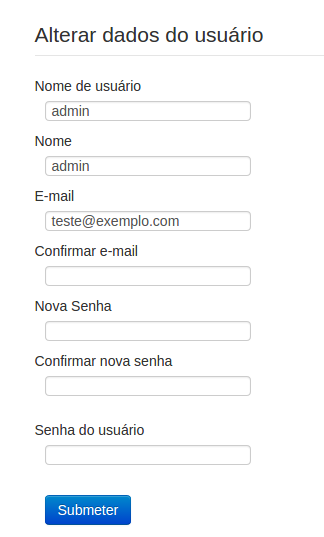
\includegraphics[scale=0.5]{images/alterardadosadmin.png}
     \caption{Alterar dados do usuário}
     \label{fig:alteraadmin}
\end{figure}

\subsubsection{Entradas}

\begin{itemize}

	\item Submeter com os campos vazios 
	\item Preencher e-mail sem formatação (ex. admin.com)
	\item Preencher todos os campos, menos confirmação de e-mail e confirmação de nova senha
	\item Preencher confirmação de e-mail e confirmação de senha com entradas diferentes dos campos de e-mail e senha
	\item Submeter formulário com a senha do administrador errada
	\item Submeter o formulário corretamente, com confirmações de e-mail e senha idênticos aos originais, senha de usuário correta, formatação do e-mail válida (admin@teste.com) e nenhum campo em branco
	
\end{itemize}

\subsubsection{Saídas}

\begin{itemize}

	\item Devem aparecer alertas ao lado de cada campo preenchido de forma (formatação) inválida ou submetido em branco
	\item Deve aparecer um alerta de erro se o e-mail e senha de confirmação não forem idênticos aos originais
	\item Deve aparecer um alerta de "senha incorreta" se a senha do usuário estiver errada
	\item Se os dados estiverem todos preenchidos de forma correta, deve aparecer uma mensagem de "Sucesso" e o usuário deve ser redirecionado para a tela inicial
	
\end{itemize}

\subsubsection{Dependência de casos de teste}
Não há dependência com nenhum outro caso de teste.

\section{Logs}\label{sec:logs}

O administrador deve poder exportar ou apagar os \textit{logs} do sistema a qualquer momento. Este arquivo contém todas as operações efetuadas pelo sistema de emissão de certificados ICPEdu até o momento em que o \textit{log} tenha sido exportado, em um formato de texto, onde cada ação é uma frase. Para fazer qualquer uma das duas operações, vá ao menu \textit{Logs}, como mostra a figura \ref{fig:logs}.

\begin{figure}[ht]
    \centering
     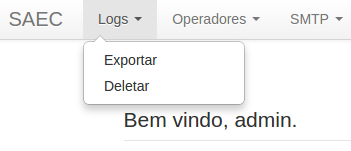
\includegraphics[scale=0.5]{images/logs.png}
     \caption{Menu Logs}
     \label{fig:logs}
\end{figure}

\subsection{Deletar Logs}

Para apagar seus \textit{logs}, basta clicar no menu \textit{Logs $>$ Deletar}. O administrador deve ser redirecionado para uma tela que pedirá sua senha para confirmar a ação.  Como esta é a única ação possível, não se faz necessário um  caso de teste específico para esta funcionalidade, basta tentar uma vez com a senha correta, e outra com a senha incorreta, onde um erro claro e preciso sobre senha de usuário inválida deve aparecer.

\subsubsection{Dependência de casos de teste}
Não há dependência com nenhum outro caso de teste.

\subsection{Exportar Logs}

Entre na funcionalidade através do menu \textit{Logs $>$ Exportar}. Exporte os \textit{logs} do usuário. Ao clicar, o download deve acontecer automaticamente. Abra o arquivo e verifique as últimas ações. Caso o \textit{log} tenha sido deletado anteriormente, esta ação deverá estar presente no arquivo. Como esta é a única ação possível, não se faz necessário um  caso de teste específico para esta funcionalidade.

\subsubsection{Dependência de casos de teste}
Não há dependência com nenhum outro caso de teste.